\section{Results of the Runtime Verified AV System}

This research provides a solution for two aspects of \acf{AV} systems: predicting accurately with perturbations to the system's inputs and safely dealing with misclassifications by the system.
The issue of input perturbations was addressed using a \acf{MNN} of different convolutional \acfp{SNN}, each \ac{SNN} working in tandem to predict more accurately.
Misclassification by the system's controller was addressed by implementing sensor fusion between cameras and \ac{LiDAR}.
This was done using a run-time enforcer that enforced a safety automaton.

To test the \ac{MNN}'s ability to deal with perturbations, the input images (taken from the \ac{VOC} 2012 and \ac{GTSRB} datasets) were perturbed by randomly replacing approximately 7\% of the image pixels with randomly coloured pixels.
Table~\ref{tbl:sign-res} shows that without perturbations, the accuracy of the \ac{MNN} was increased from 87.07\% to 93.7\% when using an enforced policy.
Table~\ref{tbl:sign-respert} shows that the accuracy of the \ac{MNN} hugely decreases when perturbations are present, from 87.07\% to 41.6\%.
However, with sensor fusion and a relative safety policy, the accuracy is increased to 90.48\%.
 
\begin{table}[h]
	\centering
	\resizebox{\textwidth}{!}{%
		\begin{tabular}{|l|l|l|l|l|l|}
			\hline
			Test case  & Person & Vehicle & Nothing of relevance & Street sign & Total \\ \hline
			Number of misclassifications & 1.23 & 3.82 & 3.27 & 4.61 & 12.93 \\ \hline 
			Caught misclassifications & 1.00 & 3.64 & 3.20 & 3.75 & 11.59 \\ \hline
			False negatives & 0.79 & 0.90 & 0.37 & 2.90 & 4.96 \\ \hline
			Missed misclassifications & 1.02 & 1.09 & 0.44 & 3.75 & 6.30 \\ \hline
		\end{tabular}%
	}
	\caption{Table showing results of the \ac{AV} prediction \ac{SNN} using the original images trained for 10000 epochs}
	\label{tbl:sign-res}
\end{table}

\begin{table}[h]
	\centering
	\resizebox{\textwidth}{!}{%
		\begin{tabular}{|p{0.17\linewidth}||p{0.17\linewidth}|p{0.17\linewidth}|p{0.17\linewidth}|p{0.17\linewidth}|}
			\hline
			Object classified & No. of misclassifications (\%) & Caught misclassifications (\%) & False negatives (\%) & Total remaining misclassifications (\%) \\ \hline
			Person & 17.01 & 17.01 & 0.00 & 0.00 \\ \hline
			Vehicle & 15.85 & 15.85 & 0.00 & 0.00 \\ \hline
			Sign & 54.46 & 54.46 & 4.84 & 4.84 \\ \hline
			Nothing & 7.83 & 7.83 & 0.00 & 0.00 \\ \hline
			All & 95.16 & 95.16 & 4.84 & 4.84 \\ \hline
		\end{tabular}%
	}
	\caption{Table showing results of the \ac{AV} prediction \ac{SNN} using perturbed images trained for 1 epochs}
	\label{tbl:sign-respert1}
\end{table}

\begin{table}[h]
	\centering
	\resizebox{\textwidth}{!}{%
		\begin{tabular}{|p{0.17\linewidth}||p{0.17\linewidth}|p{0.17\linewidth}|p{0.17\linewidth}|p{0.17\linewidth}|}
			\hline
			Object classified & No. of misclassifications (\%) & Caught misclassifications (\%) & False negatives (\%) & Total remaining misclassifications (\%) \\ \hline
			Person & 17.01 & 17.01 & 0.00 & 0.00 \\ \hline
			Vehicle & 15.85 & 15.85 & 0.00 & 0.00 \\ \hline
			Sign & 54.53 & 54.53 & 4.77 & 4.77 \\ \hline
			Nothing & 7.83 & 7.83 & 0.00 & 0.00 \\ \hline
			All & 95.23 & 95.23 & 4.77 & 4.77 \\ \hline
		\end{tabular}%
	}
	\caption{Table showing results of the \ac{AV} prediction \ac{SNN} using perturbed images trained for 10 epochs}
	\label{tbl:sign-respert10}
\end{table}

\begin{table}[h]
	\centering
	\resizebox{\textwidth}{!}{%
		\begin{tabular}{|p{0.17\linewidth}||p{0.17\linewidth}|p{0.17\linewidth}|p{0.17\linewidth}|p{0.17\linewidth}|}
			\hline
			Object classified & No. of misclassifications (\%) & Caught misclassifications (\%) & False negatives (\%) & Total remaining misclassifications (\%) \\ \hline
			Person & 7.69 & 3.01 & 0.32 & 5.01 \\ \hline
			Vehicle & 13.70 & 12.21 & 0.12 & 1.60 \\ \hline
			Sign & 56.01 & 37.24 & 1.37 & 20.14 \\ \hline
			Nothing & 7.83 & 7.83 & 0.00 & 0.00 \\ \hline
			All & 85.24 & 60.30 & 1.81 & 26.74 \\ \hline
		\end{tabular}%
	}
	\caption{Table showing results of the \ac{AV} prediction \ac{SNN} using perturbed images trained for 100 epochs}
	\label{tbl:sign-respert100}
\end{table}

\begin{table}[h]
	\centering
	\resizebox{\textwidth}{!}{%
		\begin{tabular}{|p{0.17\linewidth}||p{0.17\linewidth}|p{0.17\linewidth}|p{0.17\linewidth}|p{0.17\linewidth}|}
			\hline
			Object classified & No. of misclassifications (\%) & Caught misclassifications (\%) & False negatives (\%) & Total remaining misclassifications (\%) \\ \hline
			Person & 3.66 & 1.39 & 0.93 & 3.20 \\ \hline
			Vehicle & 9.06 & 7.00 & 0.60 & 2.67 \\ \hline
			Sign & 33.05 & 27.14 & 2.18 & 8.09 \\ \hline
			Nothing & 6.65 & 6.12 & 0.07 & 0.60 \\ \hline
			All & 52.42 & 41.65 & 3.78 & 14.55 \\ \hline
		\end{tabular}%
	}
	\caption{Table showing results of the \ac{AV} prediction \ac{SNN} using perturbed images trained for 1000 epochs}
	\label{tbl:sign-respert1000}
\end{table}

\begin{table}[h]
	\centering
	\resizebox{\textwidth}{!}{%
		\begin{tabular}{|p{0.17\linewidth}||p{0.17\linewidth}|p{0.17\linewidth}|p{0.17\linewidth}|p{0.17\linewidth}|}
			\hline
			Object classified & No. of misclassifications (\%) & Caught misclassifications (\%) & False negatives (\%) & Total remaining misclassifications (\%) \\ \hline
			Person & 4.01 & 0.72 & 0.42 & 3.71 \\ \hline
			Vehicle & 11.33 & 9.15 & 0.35 & 2.53 \\ \hline
			Sign & 44.17 & 37.61 & 1.27 & 7.83 \\ \hline
			Nothing & 7.32 & 7.00 & 0.07 & 0.39 \\ \hline
			All & 66.84 & 54.48 & 2.11 & 14.46 \\ \hline
		\end{tabular}%
	}
	\caption{Table showing results of the \ac{AV} prediction \ac{SNN} using perturbed images trained for 10000 epochs}
	\label{tbl:sign-respert10000}
\end{table}

\begin{figure}[t]
	\centering
	\scalebox{1}{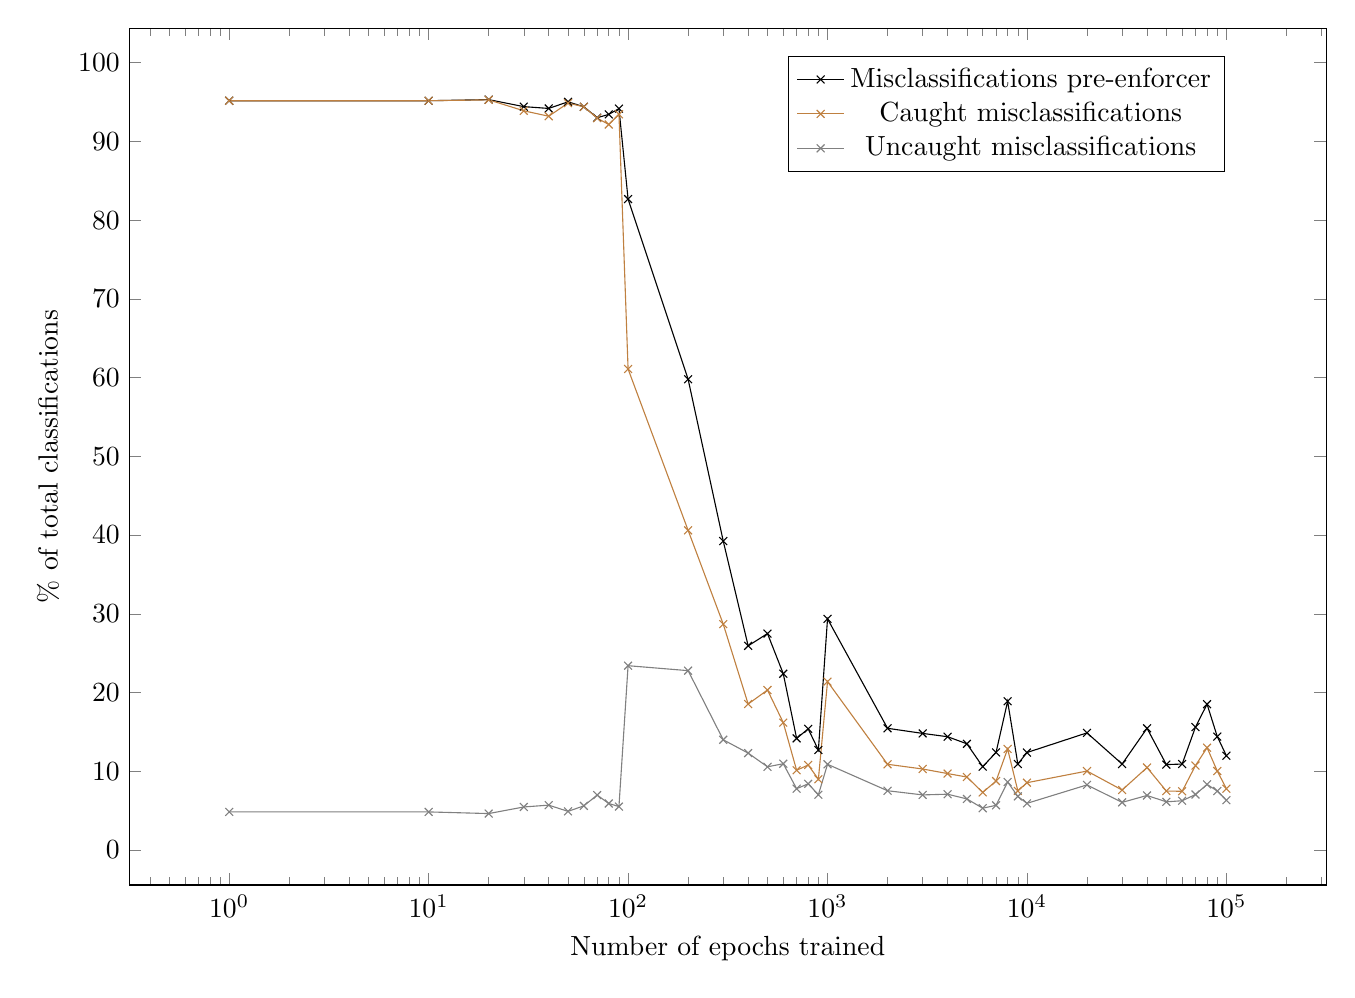
\begin{tikzpicture}
\begin{semilogxaxis}[
xlabel={Number of epochs trained},
ylabel={\% of total classifications},
x=1.1cm,
y=1.0mm, 
legend style={at={(0.55,0.9)},anchor=west}]

\addplot[color=black,mark=x] coordinates {
	(1, 95.159996)
	(10, 95.159996)
	(20, 95.300003)
	(30, 94.410004)
	(40, 94.180000)
	(50, 95.019997)
	(60, 94.389999)
	(70, 93.000000)
	(80, 93.419998)
	(90, 94.159996)
	(100, 82.669998)
	(200, 59.790001)
	(300, 39.240002)
	(400, 25.930000)
	(500, 27.490000)
	(600, 22.389999)
	(700, 14.180000)
	(800, 15.390000)
	(900, 12.700000)
	(1000, 29.359999)
	(2000, 15.460000)
	(3000, 14.810000)
	(4000, 14.390000)
	(5000, 13.490000)
	(6000, 10.590000)
	(7000, 12.400000)
	(8000, 18.889999)
	(9000, 10.920000)
	(10000, 12.380000)
	(20000, 14.880000)
	(30000, 10.920000)
	(40000, 15.460000)
	(50000, 10.850000)
	(60000, 10.920000)
	(70000, 15.620001)
	(80000, 18.520000)
	(90000, 14.410000)
	(100000, 11.980000)
};

\addplot[color=brown,mark=x] coordinates {	
	(1, 95.159996)
	(10, 95.159996)
	(20, 95.269997)
	(30, 93.880005)
	(40, 93.189995)
	(50, 94.860001)
	(60, 94.389999)
	(70, 92.950005)
	(80, 92.139999)
	(90, 93.440002)
	(100, 61.090000)
	(200, 40.599998)
	(300, 28.690001)
	(400, 18.540001)
	(500, 20.320000)
	(600, 16.180000)
	(700, 10.130000)
	(800, 10.800000)
	(900, 8.990000)
	(1000, 21.389999)
	(2000, 10.890000)
	(3000, 10.290000)
	(4000, 9.710000)
	(5000, 9.270000)
	(6000, 7.320000)
	(7000, 8.760000)
	(8000, 12.840000)
	(9000, 7.510000)
	(10000, 8.550000)
	(20000, 10.030000)
	(30000, 7.620000)
	(40000, 10.480000)
	(50000, 7.490000)
	(60000, 7.460000)
	(70000, 10.730000)
	(80000, 13.000000)
	(90000, 10.030000)
	(100000, 7.790000)
};

\addplot[color=gray,mark=x] coordinates {
	(1, 4.840000)
	(10, 4.840000)
	(20, 4.630000)
	(30, 5.470000)
	(40, 5.700000)
	(50, 4.910000)
	(60, 5.610000)
	(70, 6.980000)
	(80, 5.910000)
	(90, 5.520000)
	(100, 23.410000)
	(200, 22.780001)
	(300, 14.000000)
	(400, 12.310000)
	(500, 10.570000)
	(600, 10.960000)
	(700, 7.790000)
	(800, 8.410000)
	(900, 7.020000)
	(1000, 10.890000)
	(2000, 7.530000)
	(3000, 7.000000)
	(4000, 7.090000)
	(5000, 6.490000)
	(6000, 5.310000)
	(7000, 5.680000)
	(8000, 8.640000)
	(9000, 6.810000)
	(10000, 5.930000)
	(20000, 8.270000)
	(30000, 6.050000)
	(40000, 6.930000)
	(50000, 6.120000)
	(60000, 6.260000)
	(70000, 7.050000)
	(80000, 8.340000)
	(90000, 7.490000)
	(100000, 6.330000)
};

\legend{Misclassifications pre-enforcer, Caught misclassifications, Uncaught misclassifications}
\end{semilogxaxis}%
\end{tikzpicture}%}
	\caption{Line graph showing the performance of the system trained over an increasing amount of epochs using unperturbed inputs \label{fig:sign-graph}}
\end{figure}

\begin{figure}[t]
	\centering
	\scalebox{1}{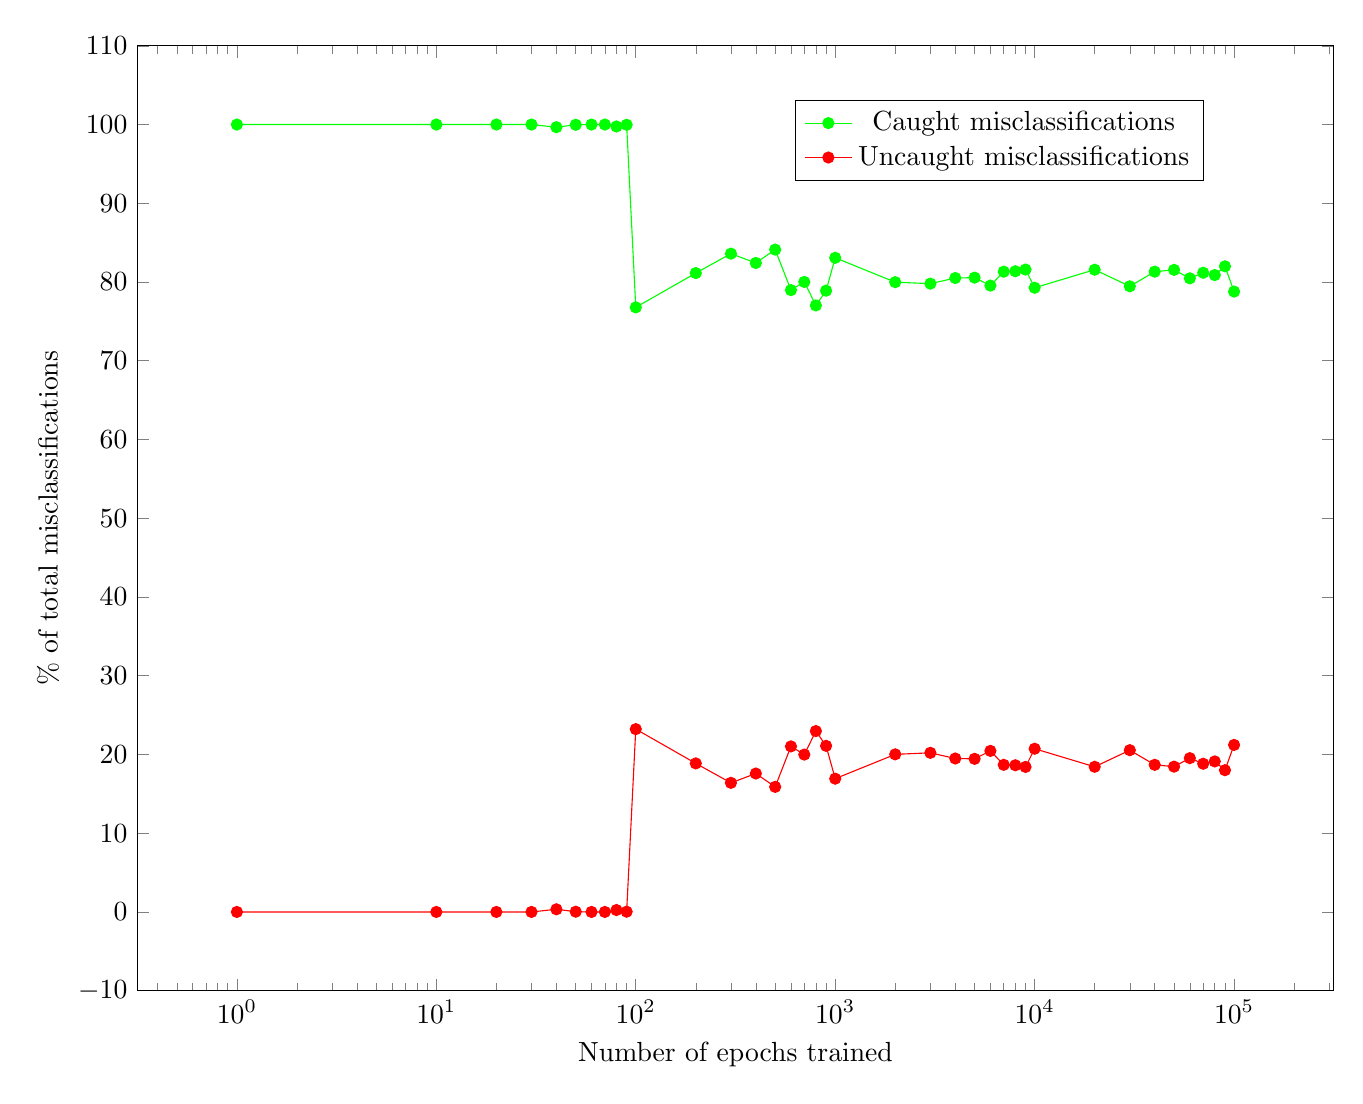
\begin{tikzpicture}
\begin{semilogxaxis}[
xlabel={Number of epochs trained},
ylabel={\% of total misclassifications},
x=1.1cm,
y=1.0mm, 
legend style={at={(0.55,0.9)},anchor=west}]

\addplot[color=green,mark=*] coordinates {	
	(1, 100.000000)
	(10, 100.000000)
	(20, 100.000000)
	(30, 100.000000)
	(40, 99.662552)
	(50, 99.968597)
	(60, 100.000000)
	(70, 100.000000)
	(80, 99.758133)
	(90, 99.968475)
	(100, 76.780945)
	(200, 81.134331)
	(300, 83.604851)
	(400, 82.419716)
	(500, 84.116234)
	(600, 78.973373)
	(700, 80.015221)
	(800, 77.028572)
	(900, 78.905663)
	(1000, 83.074722)
	(2000, 79.983315)
	(3000, 79.792389)
	(4000, 80.510559)
	(5000, 80.555107)
	(6000, 79.547066)
	(7000, 81.314125)
	(8000, 81.369659)
	(9000, 81.582603)
	(10000, 79.271027)
	(20000, 81.565376)
	(30000, 79.456421)
	(40000, 81.315414)
	(50000, 81.545204)
	(60000, 80.468216)
	(70000, 81.178162)
	(80000, 80.884285)
	(90000, 81.995102)
	(100000, 78.786835)
};

\addplot[color=red,mark=*] coordinates {
	(1, 0.000000)
	(10, 0.000000)
	(20, 0.000000)
	(30, 0.000000)
	(40, 0.337446)
	(50, 0.031402)
	(60, 0.000000)
	(70, 0.000000)
	(80, 0.241872)
	(90, 0.031525)
	(100, 23.219051)
	(200, 18.865665)
	(300, 16.395145)
	(400, 17.580284)
	(500, 15.883766)
	(600, 21.026627)
	(700, 19.984774)
	(800, 22.971428)
	(900, 21.094332)
	(1000, 16.925280)
	(2000, 20.016680)
	(3000, 20.207613)
	(4000, 19.489441)
	(5000, 19.444899)
	(6000, 20.452932)
	(7000, 18.685873)
	(8000, 18.630341)
	(9000, 18.417391)
	(10000, 20.728970)
	(20000, 18.434624)
	(30000, 20.543579)
	(40000, 18.684584)
	(50000, 18.454794)
	(60000, 19.531784)
	(70000, 18.821840)
	(80000, 19.115713)
	(90000, 18.004898)
	(100000, 21.213161)
};

\legend{Caught misclassifications, Uncaught misclassifications}
\end{semilogxaxis}%
\end{tikzpicture}%}
	\caption{Line graph showing the number of misclassifications made by the system with perturbed inputs \label{fig:sign-graphpert}}
\end{figure}

\todo{Add results for multiple epochs}
\todo{Add table showing how \ac{MNN} affects the prediction accuracy}